\section{Concept mass estimation} \label{ch:strucmass}
It is essential that decelerator concepts are analyzed in terms of mass to fully appreciate the mass benefits of a certain decelerator concept. A reduced decelerator mass allows for a larger payload mass to be taken on board, since launcher mass capability is intended to be fully fulfilled. It is therefore essential that the concept selection takes into account decelerator mass. To this end a mass estimation tool is constructed to provide a first estimate of concept mass for an informed decision in the concept trade-off.

This chapter is structured in the following manner. Firstly, the purpose of tool development is outlined in section \ref{sec:strucpurp} to prevent a clear view of the required tool output. Based hereupon, a tool is constructed using a number of methods as described in section \ref{sec:strucmeth}. Verification and validation activities are described in section \ref{sec:strucvv}. The tools are then applied firstly to compare the selected decelerator concepts in terms of mass, as described in section \ref{sec:struccc}, secondly to provide an overview of the effect of materials choice on decelerator mass, as described in section \ref{sec:strucmat}, and lastly to perform a sensitivity analysis, as described in section \ref{sec:strucsens}. Conclusions are formulated in section \ref{sec:strucconc}.

\subsection{Purpose of tool development}\label{sec:strucpurp}
The purpose of the tool is twofold:
\begin{itemize}
\item To obtain a decelerator mass estimate for each of the five concepts in order to evaluate their mass performance;
\item To investigate the effect of concept design variables on decelerator mass;
\end{itemize}
The former is investigated primarily in section \ref{sec:struccc}, where the decelerator concepts are evaluated for their mass performance, while the latter is investigated in sections \ref{sec:strucmat} and \ref{sec:strucsens}. The mass estimate is primarily intended for relative comparison in this design phase, closed by the \acrfull{mtr}. It remains, however, a valuable tool in analysis and design of the selected concept by providing an actual mass estimate for a selection of design variables. This selection of design variables can thus be made using the mass estimate provided by the tool, by a minimization of decelerator mass.

\subsection{Methods for mass estimation}\label{sec:strucmeth}
The structural mass estimation is done using two separate methods: mass estimates based on reference missions and mass estimates based on structural models. The latter will be used for the analysis of the structural mass for the four inflatable concepts: the stacked toroid, isotensoid, tension cone and trailing configurations. For these concepts few reference missions are available for an adequate mass estimation and the availability of parametric mass modeling \cite{Anderson1969, Samareh2011} make structures-based models the preferred option. Historically, rigid re-entry vehicles have been applied numerous times and a mass estimation can be done on the base of reference missions. These mass estimation methods are presented hereafter.

\subsubsection{Isotensoid mass estimation}
%los maar op
For the mass estimation based on the structural models two different methods are employed. First off, for the isotensoid and trailing concepts Anderson \cite{Anderson1969} hsa developed a structural merit model. Modern implementations, as presented by for example Miller \cite{Miller2014}, use this mass estimation for current investigations in the feasibility of aerodynamic decelerators. The mass estimation presented by Anderson for the isotensoid concept considers a model inflated by ram-air, an inflation method commonly considered for isotensoid structures \cite{Smith2011}. For the trailing ballute configuration Anderson considers a ram-air inflated structure as well, similar to the isotensoid configuration. For the trailing configuration different models may be considered and a ballute in the from of a "donut" is also commonly analysed. 
Andersons model provide the structural mass estimation as a single variable for the whole isotensoid or ballute configuration. The mass estimation is presented in the from of the \gls{bc} of the structure. This value can consequently be used for a mass estimation of the isotensoid or ballute configurations.

Andersons model is provided in two forms: First of a basic model requiring as input the peak dynamic pressure (\gls{sym:q}) and the frontal surface area (\gls{sym:A}) which can also be implicitly considered using the outer diameter. Moreover decelerator material properties are considered using the materials aerial density (\gls{sym:df}). Andersons model assumes the use of a single material for the whole decelerator design. For the computation of the aerial density a minimum gage thickness is considered.

 It must be noted that this simple model implicitly includes as set value for the drag coefficient (\gls{sym:CD}). The full model requires a complete set of parameters which is provided by \cite{Anderson1969} and allows control of the drag coefficient as well which can be considered useful for a sensitivity analysis. More detailed analysis of other parameters are not considered at this in the design. A more detailed estimation is not desired as it requires a detailed configuration of the concept
%tot hier
\subsubsection{Stacked toroid, tension cone and trailing ballute mass estimation}
Mass estimation for stacked toroid, tension cone and trailing \gls{iad} configurations is performed by the method outlined in Ref.\cite{Samareh2011}. Similar to the model by Anderson, it introduces a figure of merit by defining a dimensionless mass efficiency parameter \gls{sym:mbar}, defined as:
\begin{equation}
\gls{sym:mbar} = \frac{\gls{sym:m}}{\gls{sym:mfactor}}
\label{eq:dimmass}
\end{equation}
where \gls{sym:mfactor} is defined by the following equation
\begin{equation}
\gls{sym:mfactor} = \frac{\gls{sym:A_iad} \gls{sym:CD} \gls{sym:q}}{\gls{sym:ge}}
\label{eq:mfactor}
\end{equation}
A concept having a high dimensionless mass efficiency parameter may be interpreted as a concept having a high IAD areal density scaled by dynamic pressure. It is desirable to have this parameter as small as possible, to effect a larger area capable of withstanding greater dynamic pressure with the lowest possible mass.

As inputs, the mass estimation requires \cite{Samareh2011}:
\begin{itemize}
\item Decelerator configuration (stacked toroid/tension cone/trailing ballute);
\item The material properties used corresponding to the material used for the inflatable structure; 
\item A specification of the material used for the wall lay-up. Options are solely a film, thus one material that does not require an additional coating and gas barrier, a film complemented by a coating but does require a gas barrier and a fiber reinforced fabric requiring both coating and a gas barrier;
\item The centerbody and deployed diameter;
\item The half-cone angle \gls{sym:theta} (depicted in Figure 2 of \cite[p.7]{Samareh2011});
\item The number of toroids for a stacked toroid configuration;
\item The reigning static and dynamic pressure and vehicle drag coefficient;
\item The diameter of tori;
\item Inflation gas temperature and molecular weight;
\item The number of radial straps;
\item Vehicle (characteristic) length;
\item Margins and knockdown factors accounting for seams and stress concentrations. These are taken as defined in tabular form on page 16 of Ref.\cite{Samareh2011}.
\end{itemize}

Based on these inputs, the mass estimation procedure yields the following outputs \cite{Samareh2011}:
\begin{itemize}
\item Mass of reinforcing elements (radial and axial straps);
\item Mass of flexible bladder material;
\item Mass of inflation gas;
\item Inflation gas pressure;
\item Mass of inflation system;
\item Total mass.
\end{itemize}
All outputs can be given either in dimensionless or dimensional forms, with conversion from one to the other performed through Eq.\ref{eq:dimmass}. A \texttt{MATLAB} tool has been constructed that allows varying these inputs and provides a parametric estimation of the decelerator mass for each of these three inflatable concepts. This allows the investigation of the effect of changing input parameters on the various output parameters. Key output parameter at this stage is the total mass, for the purpose of concept comparison in terms of mass performance. Moreover, inflation gas pressure and inflation gas mass provide a benchmark for investigating the effect of using different inflation gases.




\subsubsection{Rigid structure mass estimation}

\subsection{Tool verification and validation}\label{sec:strucvv}
Verification and validation of the mass estimation tools is performed as follows. These activities can be divided primarily into the verification and validation of the mass estimation tool adapted from Samareh \cite{Samareh2011} for stacked toroid, tension cone and trailing \gls{iad} devices on one hand and verification and validation of the mass estimation tool adapted from Anderson \cite{Anderson1969} for isotensoid and trailing \gls{iad} devices on the other hand. The rigid concept is analysed using an empirical model by Steinfeldt \cite{Steinfeldt2009}.

\subsubsection{Anderson inflatable mass estimation method}
In order to verify the implementation of the mass estimation tool presented by Anderson in Ref. \cite{Anderson1969} the tools results were compared to the results presented in the paper by Anderson. The full estimation model was implemented and consequently checked with the coefficients of the simplified model coefficients presented on page 16 and 20 of Ref. \cite{Anderson1969}. Finally the results of the full model were compared with the results of the merit function for the attached isotensoid on page 30 of Ref. \cite{Anderson1969}. No errors were observed in the significant digits of both estimates. The mass estimates were further verified using the results presented by Clark on page 11 in Ref. \cite{Clark2009}, similarly yielding no errors detectable within the range of significant digits.

No additional validation of the mass estimation model by Anderson \cite{Anderson1969} was performed, by the absence of experimental testing of attached isotensoid concepts. This absence is reflected to some extent by the figure on page 3 of Ref.\cite{Smith2010}, from which it may be deduced that isotensoids have been flown very seldom from a historical perspective.

\subsubsection{Samareh inflatable mass estimation method}
In order to verify that the mass estimation method described in Ref.\cite{Samareh2011} has been correctly implemented, results for the nine sample cases presented on page 16 of Ref.\cite{Samareh2011} have been checked. These nine sample cases were implemented by choosing the input parameters as given in tabular form (Tables 4 and 5) on page 16 of Ref.\cite{Samareh2011} and the output parameters, primarily component masses and geometric quantities, were compared. A maximum error of 3 $\%$ in terms of total mass was obtained; a maximum error of 2 $\%$ in component masses. These errors are deemed sufficiently small to verify successful implementation of the mass estimation method.

Validation is performed indirectly: the method \cite{Samareh2011} has been applied in the \gls{edlsa} project \cite{Cianciolo2010}, where it was shown to yield results conforming well to the outcomes of high-fidelity \gls{fea}. The used \gls{fea} is a validated tool \cite{Cianciolo2010} and thereby the method outlined in Ref.\cite{Samareh2011} has been validated through comparison with a high-fidelity validated model. Moreover, the expression for minimum inflation pressure obtained by Samareh has been found to be in correspondence with Yamada et al \cite{Yamada2009}, Clark \cite{Clark2009} and Brown \cite{Brown2009}.

A qualitative check on the results obtained by this mass estimation method is performed by assessing the relations found in section \ref{sec:strucmat} and \ref{sec:strucsens} for their conformance to expectations and other literature on inflatable aerodynamic decelerators. The outcomes hereof are reflected by the discussions in these respective sections.


\subsection{Rigid mass estimation method}
The rigid mass estimation is one that is performed on the basis of reference missions. Simple models which are suggested by Steinfeldt \cite{Steinfeldt2009} are employed for which the relations are checked with the results on page 8 of \cite{Steinfeldt2009} and page 3 of \cite{Laub2004}. The result were found to match.

For the rigid concepts validation is a important factor. Since the rigid mass estimation is based on reference missions with a empirical model the quality of the fit is one of crucial importance.
Steinfeldt provides three mass estimates for different components of a hypersonic decelerator. These are also further detailed in section \ref{sec:rigid}.

\begin{itemize}
\item A forebody thermal protection system mass estimate. This value is based on eight reference missions and the models remain within 4\%.
\item A forebody structural mass estimate based on six reference missions errors remain within 3\%.
\item A combined structural and thermal backshell mass estimate on the basis of two reference missions of which the the value is a weighted average
\end{itemize}

The errors provided above are percentages of the total spacecraft mass (\gls{m0}). Given the limited amount of reference vehicles used, especially for the backshell mass estimate, the validity must be appropriately considered whenever the model is used. It can however serve as indicative value taking the error of the model into account.
\subsection{Concept comparison}\label{sec:struccc}
In terms of comparing the decelerator concepts in terms of mass, the total decelerator mass as yielded by the methods outlined in section \ref{sec:strucmeth} is computed for each of the five concepts. Due to the limited applicability of each of the methods used, a necessity is the use of multiple methods: the method by Samareh \cite{Samareh2011} for the mass estimation of stacked toroid, tension cone and trailing \gls{iad} concepts; the method by Anderson \cite{Anderson1969} for the mass estimation of the isotensoid and the reference method for the mass estimation of the rigid concept. 

[ADD MORE]
\subsection{Structural materials comparison}\label{sec:strucmat}
Materials for inflatable structures are typically high-performance high-temperature-resistant woven fabrics, supplemented by coatings to reduce porosity \cite{Jenkins2001}. These materials are required to be lightweight, strong, heat-resistant and flexible for application in \glspl{hiad} \cite{Samareh2010}. On one hand there are heritage materials, such as Kapton, but for current \gls{hiad} missions these have been replaced by up-and-coming materials, such as Vectran and PBO Zylon \cite{Dillman2012,  Smith2010}. Key driver for the use of these materials is a high specific strength compared to metals (e.g. aluminium) \cite{Samareh2010}. 

An overview of materials, and their key properties, suitable for \gls{hiad} application is given in Table \ref{table:strucmatoverview}. 

\begin{table}[h]
\begin{tabular}{lllllllllllll}
\caption{Overview of candidate materials for \gls{hiad} application}
\textbf{Material}            & \textbf{Type of material {[}-{]}} & \textbf{Density {[}kg/m\textasciicircum 3{]}} & \textbf{Areal density {[}kg/m\textasciicircum 2{]}} & \textbf{Elongation at break {[}\%{]}} & \textbf{Specific strength {[}kN km/kg{]}} & \textbf{Breaking strength {[}km{]}} & \textbf{Breaking tenacity {[}g/denier{]}} & \textbf{Tensile strength {[}GPa{]}} & \textbf{Young's Modulus {[}GPa{]}} & \textbf{Poisson's Ratio {[}-{]}} & \textbf{From} &  \\
Kapton Type 100 HN           & Polyimide film                    & 1420                                          &                                                     & 72                                    & 163                                       & 16.6                                & 1.84                                      & 0.231                               & 2.5                                & 0.34                             &               &  \\
Kevlar 29 (1500 denier)      & Aramid fiber                      & 1440                                          & 0.2080                                              & 3.6                                   & 2031                                      & 207.0                               & 23.00                                     & 2.92                                & 70.5                               & 0.36                             &               &  \\
Kevlar 49 (1140 denier)      & Aramid fiber                      & 1440                                          & 0.1810                                              & 2.4                                   & 2084                                      & 212.4                               & 23.60                                     & 3.00                                & 112.4                              & 0.36                             &               &  \\
Nomex Type 430 (1200 denier) & Aramid fiber                      & 1380                                          & 0.4001                                              & 30.5                                  & 441                                       & 45.0                                & 5.00                                      & 0.61                                & 11.45                              &                                  &               &  \\
PBO Zylon AS                 & Polybenzoxazole fiber             & 1540                                          &                                                     & 3.5                                   & 3766                                      & 383.9                               & 42.66                                     & 5.80                                & 180.0                              &                                  &               &  \\
Spectra 2000 (100 denier)    & Polyethylene fiber                & 970                                           &                                                     & 3                                     & 3443                                      & 351.0                               & 39.00                                     & 3.34                                & 124.0                              &                                  &               &  \\
Technora                     & Aramid fiber                      & 1390                                          &                                                     & 4.4                                   & 2158                                      & 220.0                               & 24.45                                     & 3.00                                & 70.0                               &                                  &               &  \\
Upilex-25S                   & Polyimide film                    & 1470                                          & 0.3778                                              & 42                                    & 354                                       & 36.1                                & 4.01                                      & 0.52                                & 9.1                                &                                  &               &  \\
Vectran HT                   & Liquid Crystal Polymer fiber      & 1410                                          & 0.2780                                              & 4.3                                   & 2270                                      & 229                                 & 25.44                                     & 3.20                                & 75.0                               &                                  &               & 
\end{tabular}
\label{table:strucmatoverview}
\end{table}

[TABLE NEEDS ADJUSTMENT]


\subsection{Sensitivity analysis}\label{sec:strucsens}
This section provides an indication of the effect of changing design parameters on one hand and external parameters on the other hand on the total structural decelerator mass and mass efficiency. Design parameters are primarily half-cone angle \gls{sym:theta}, drag coefficient \gls{sym:CD} and outer diameter \gls{sym:Do}. Primary external factor is the peak dynamic pressure. These parameters are evaluated with respect to their effect on decelerator structural mass, either in terms of ballistic coefficient or total mass. In addition, inflation gas molar mass and temperature are investigated for their effect on inflation gas mass and the number of toroids is investigated for the effect on the stacked toroid configuration. This indication is primarily useful to provide a good starting point for concept design in terms of the investigated design parameters and to quantify benefits associated with certain design concepts. 

Due to the limitations imposed by the mass estimation model for the isotensoid \cite{Anderson1969}, the sensitivity of isotensoid structural mass to these parameters can only be investigated in a limited manner. The more extensive model for the other three inflatable concepts \cite{Samareh2011} allows for a more involved sensitivity analysis.

\subsubsection{Inflation gas mass}
Stacked toroid, tension cone and trailing ballute configurations rely on the use of internal pressure to provide the structural rigidity required from the inflatable structure. The isotensoid uses ram-air to inflate itself and hence does not require inflation gas to be taken on-board for inflation purposes. In the mass estimation model, adapted from Samareh \cite{Samareh2011}, the inflation gas is characterized primarily by its operating temperature (in Kelvin or degrees Celsius) and its molar mass (in kilogram per mole). Inflation gas mass as a function of these two variables is displayed in Fig.\ref{fig:inflmass}

\begin{figure}[H]
\hspace{-5mm}
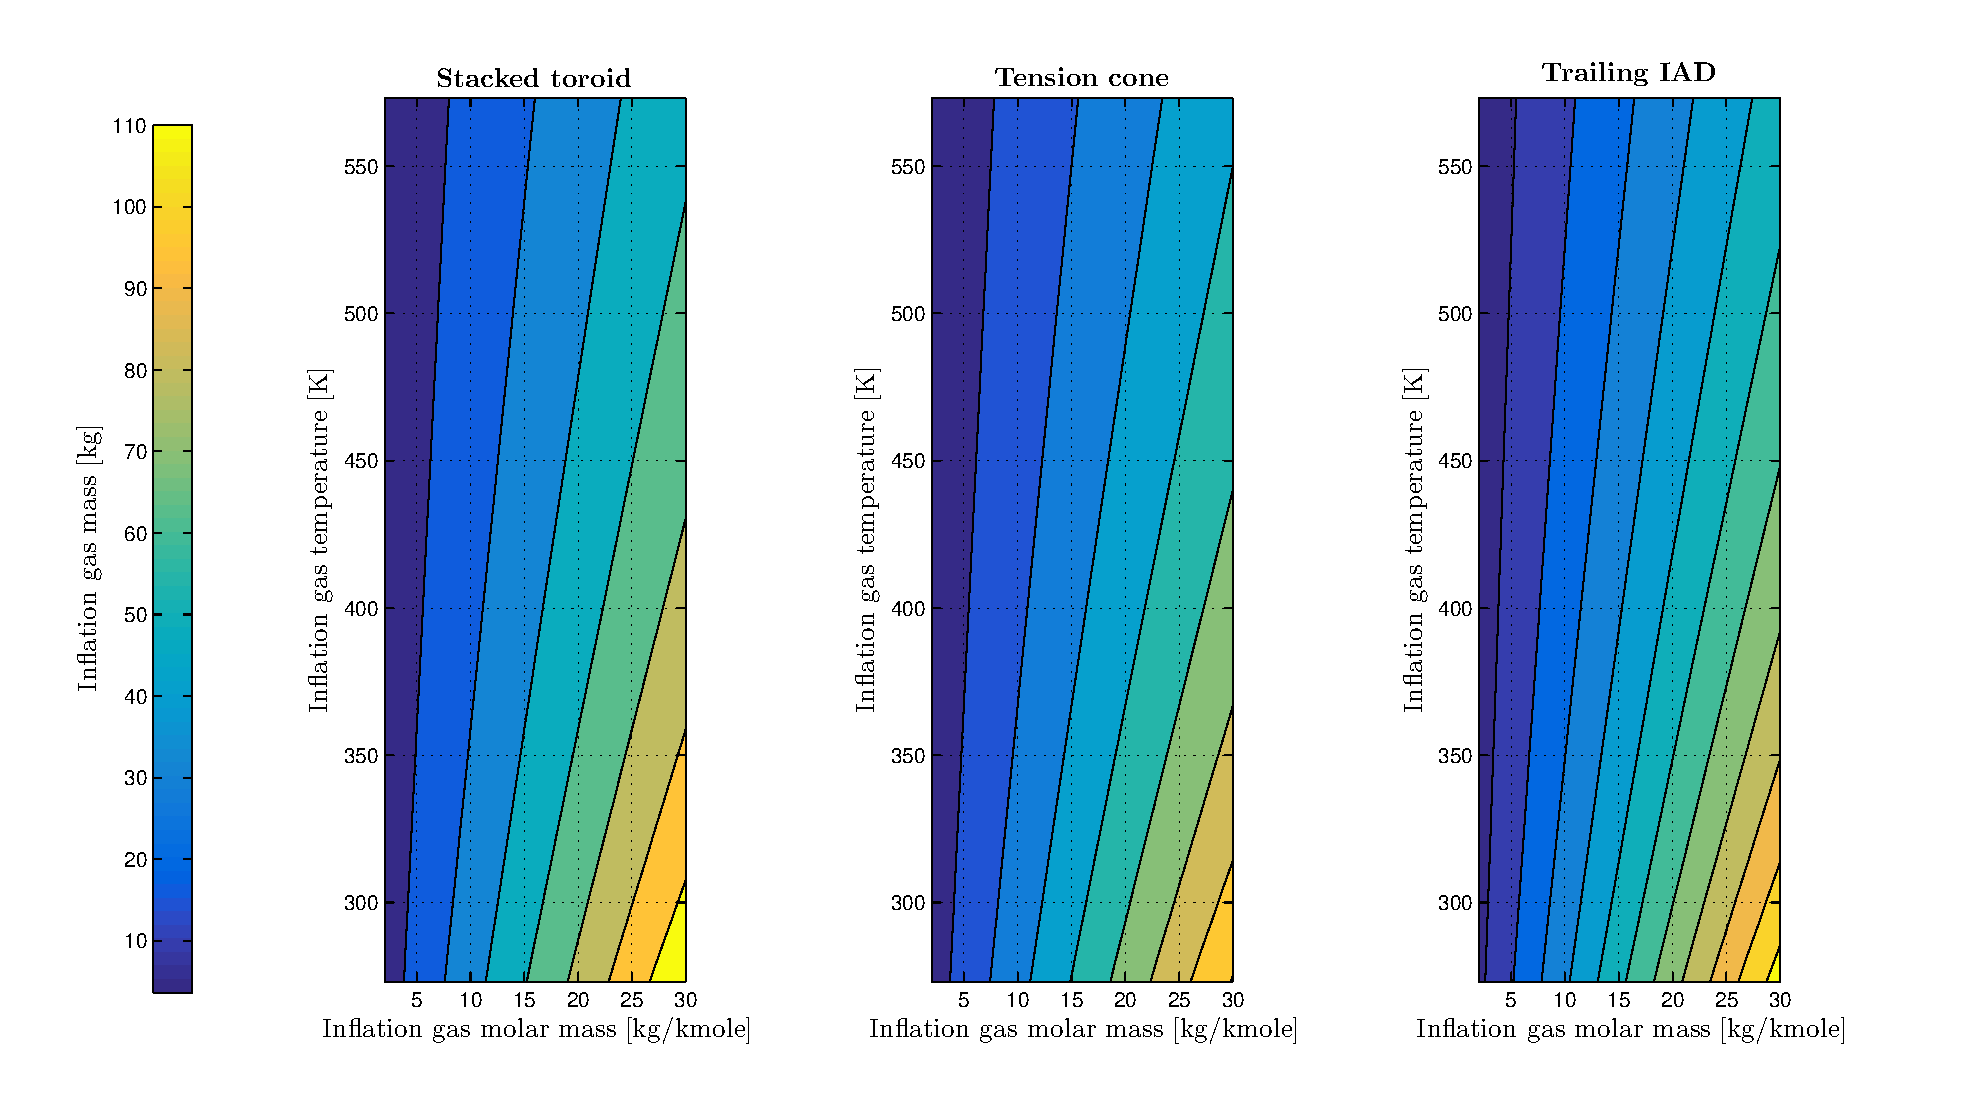
\includegraphics[width = 1.1\textwidth]{Figure/gas_temp_mass.eps}
\caption{Inflation gas mass as a function of gas temperature and molar mass of the stacked toroid, tension cone and trailing ballute configurations}
\label{fig:inflmass}
\end{figure}

Fig.\ref{fig:inflmass} confirms that a denser gas, characterized by a higher molar mass, yields a larger inflation gas mass. An overview of gas generator types and their output is given on page 7 by Brown \cite{Brown2003}. A typical molar mass is that of nitrogen, 22 [$\frac{kg}{mole}$], used in the IRVE satellites \cite{Dillman2012}. It should be noted that inflation system mass is typically estimated as a percentage of inflation gas mass. Total inflation system mass, thus consisting of inflation system and inflation gas mass, will therefore not be as low as suggested by Fig.\ref{fig:inflmass} for low molar mass inflation gases, but it will typically be higher by requiring a heavier inflation system \cite{Brown2003}. Inflation gas mass decreases for an increasing inflation gas temperature, again conforming to expectations. Via the ideal gas law the mass occupied by a certain number of moles of inflation gas will increase for a decreasing temperature through an increased gas density \cite{AndersonJr.2007}.

\subsubsection{Number of toroids for the stacked toroid configuration}
The stacked toroid features a number of toroids that are inflated. To investigate the effect of the number of toroids on total structural decelerator mass, the two are plotted against one another in Fig.\ref{fig:toro}. 

\begin{figure}[H]
\centering
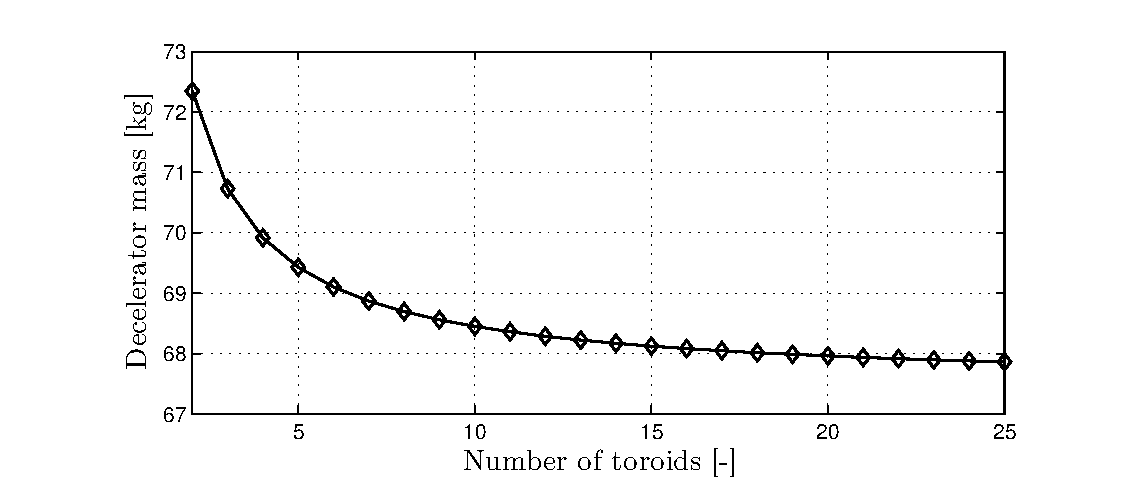
\includegraphics[width = 1.0\textwidth]{Figure/mass_toroids.eps}
\caption{Decelerator structural mass as a function of the number of toroids for the stacked toroid configuration}
\label{fig:toro}
\end{figure}

From Fig.\ref{fig:toro}, it may be observed that stacked toroid structural mass decreases for an increasing number of toroids. The decrease is, however, so slight as to be insignificant. A mass decrease of approximately 4 $\%$ is effected by an increase from one to five toroids; a decrease of approximately 5 $\%$ for an increase from one to ten toroids. As the number of toroids is increased beyond ten, mass is more or less constant. Total structural decelerator mass is therefore deemed indifferent to the number of toroids. Care should still be taken to attach too much value to the results yielded by the model, given its limited fidelity.

\subsubsection{Inflatable decelerator diameter}
Figures \ref{fig:mass_dia} and \ref{fig:bc_dia} illustrate the effect of a change in inflatable decelerator diameter on its structural mass. Fig.\ref{fig:mass_dia} illustrates that an increase in deployed diameter, given a certain peak dynamic pressure and drag coefficient, effects an exponential increase in decelerator mass. This increase is significant, adding as much as 33 $\%$ of structural mass for a tension cone for an increase in diameter from 13 to 14 [m], for a peak dynamic pressure of 3000 [Pa] and a drag coefficient of 1.5 [-]; the other concepts exhibit similar increases. A better estimate of the mass-effectiveness for an increasing diameter is given by Fig.\ref{fig:bc_dia}, which displays the ballistic coefficient of the decelerator, taking into account only its structural mass. This figure shows that the ballistic coefficient increases with increasing diameter for stacked toroid, tension cone and trailing ballute, denoting that decelerator structural mass increases more than its decelerating capability (the product of \gls{sym:CD} and \gls{sym:A_iad}) and thus that it becomes less mass-effective for an increasing deployed diameter. For the isotensoid, [ALEXANDER MINIMUM GAGE ISOTENSOID UITLEG]

\begin{figure}[H]
\centering
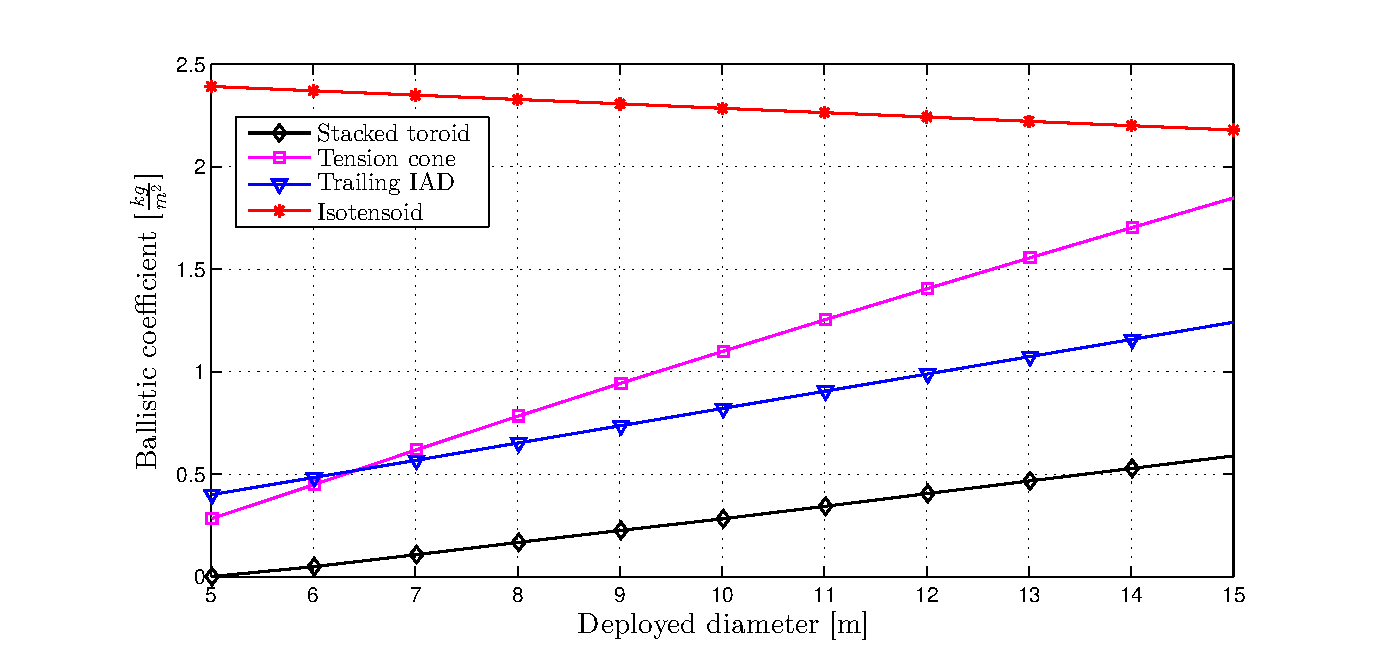
\includegraphics[width = 1.0\textwidth]{Figure/bc_dia.eps}
\caption{Decelerator structural ballistic coefficient as a function of deployed diameter of inflatable concepts}
\label{fig:bc_dia}
\end{figure}

\subsubsection{a}

\begin{figure}[H]
\centering
\includegraphics[width = 1.0\textwidth]{Figure/mass_theta_cd.eps}
\caption{Decelerator structural ballistic coefficient as a function of deployed diameter of inflatable concepts}
\label{fig:mass_theta_cd}
\end{figure}
\subsection{Conclusion}\label{sec:strucconc}

